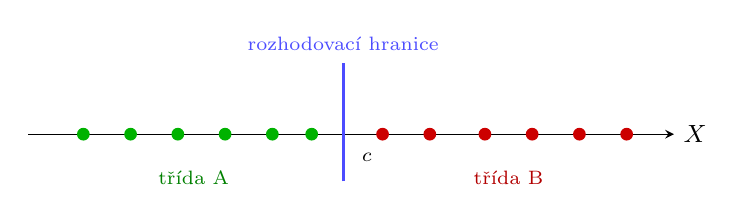
\begin{tikzpicture}[x=1cm,y=1cm,>=stealth]

    \draw[->] (0,0) -- (8.2,0)
        node[right, font=\small] {$X$};

    \draw[very thick, blue!70]
        (4,-0.6) -- (4,0.9);

    \node[font=\scriptsize, blue!70]
        at (4,1.15) {rozhodovací hranice};

    \foreach \x in {0.7,1.3,1.9,2.5,3.1,3.6}{
        \fill[green!70!black] (\x,0) circle (2.3pt);
    }

    \foreach \x in {4.5,5.1,5.8,6.4,7.0,7.6}{
        \fill[red!80!black] (\x,0) circle (2.3pt);
    }

    \node[font=\scriptsize, green!50!black]
        at (2.1,-0.55) {třída A};

    \node[font=\scriptsize, red!70!black]
        at (6.1,-0.55) {třída B};

    \node[font=\scriptsize]
        at (4.3,-0.3) {$c$};

\end{tikzpicture}
